% -------------------------------------------------------------------------------
% Name:         main.tex
% Author:      	@utahkaA (Twitter, GitHub, and so on...)
% Created:     	Jun 23rd, 2016
% Last Date:   	Jun 23rd, 2016
% Note:         xxxxx
% -------------------------------------------------------------------------------
\documentclass[a4jsme]{jsmepaper}
\usepackage[dvipdfmx]{graphicx}
\usepackage{fancyhdr}
\usepackage{epic,eepic}
%
%  Created by Ryou-Watanabe on 17/07/06.
%
\makeatletter
\renewcommand{\subsection}{%
  \@startsection{subsection}%
  {1}%
  {\z@}%
  {.5\Cvs \@plus.5\Cdp \@minus.2\Cdp}%
  {.2\Cvs \@plus.3\Cdp}%
  {\reset@font\normalsize\bfseries}%
}
\makeatother


\thispagestyle{fancy}
\lhead{\gt \normalsize 2017年度前期ゼミナール中間報告書}
\renewcommand{\headrulewidth}{0pt}
\cfoot{\thepage}
%\pagestyle{empty}

\jtitle{ゼミナール報告書テンプレに関するサンプル}
\etitle{Seminar template in OKLAB}
\jauthor{
  1426xxx\ \
  氏名
}
\eauthor{
  Write your name in roman letters
}
\jaffiliation{
  & 指導教員:大川 茂樹
}
% 著者の所属の英文
% \eaffiliation{
%     $^{*3}$  □□ Engineering, □□ University \\
%     address
%     }
% 主著者の所属の英文
%\email  {□□□□@□□□□□□}
% 原稿の事前講演など。無い時はコメントアウト
% \presentation{    年 月  日 }
% 原稿受付日(省略すると本日)
\date{\today}
% 英文の概要
\abstract{
  xxxxxxxxxxxxxxxxxxxxxxxxxxxxxxxxxxxxxxxxxxxxxxxxxxxxxxxxxxxxxxxxxxxxxxxxxxxxxx
\abind
  xxxxxxxxxxxxxxxxxxxxxxxxxxxxxxxxxxxxxxxxxxxxxxxxxxxxxxxxxxxxxxxxxxxxxxxxxxxxxx
}
% キーワード
\keywords{xxxx,yyyy,zzzz}

\begin{document}
\maketitle
\thispagestyle{fancy}

\section*{はじめに}
はじめにを書く場所


\section{研究目的}

画像は,eps とか使うより,png でいいと思います.
\begin{figure}[htbp]
  \begin{center}
    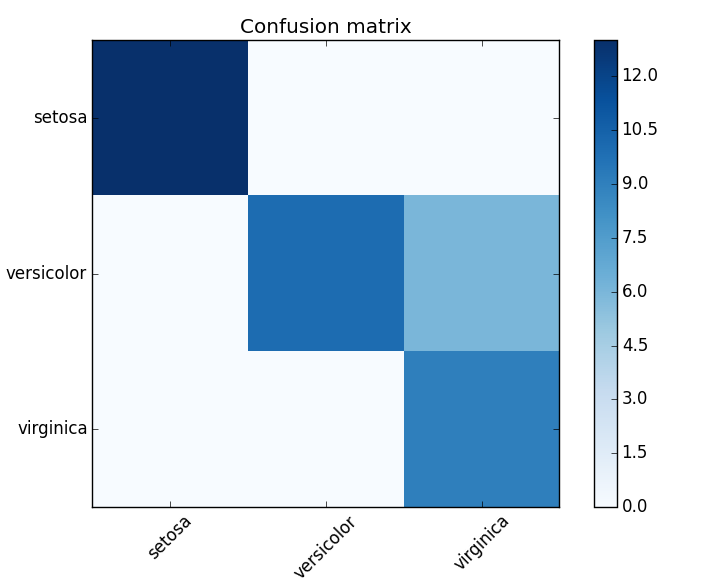
\includegraphics[width=7cm]{img/iris_confusion_matrix.png}
    \caption{アヤメの品種を識別した際の混合行列}
    \label{fig:one}
  \end{center}
\end{figure}\

\section{関連研究}
\subsection{第2章第1節です。\\}

\section{研究方法}
\subsection{第3章第1節です}
\subsection{第3章第2節です}

\section{結果と考察}

\section{今後の方針}


\section*{おわりに}





{\small
\begin{thebibliography}{99}
  \bibitem{Bisot16}
    V. Bisot, R. Serizel, S. Essid, and G. Richard.
    ``Supervised Nonnegative Matrix Factorization for acoustic scene classification,"
    {\it IEEE AASP Challenge on Detection and Classification of Acoustic Scenes and Events (DCASE)},
    2016.
  \bibitem{Roma13}
    G.Roma, W. Nogueira, P. Herrera, and R. de Boronat.
    ``Recurrence quantification analysis features for auditory scene classification",
    {\it IEEE Workshop on Applicat. Signal Process. Audio Acoust.},
    New Paltz, NY, USA, pp. 1-4, 2013.
\end{thebibliography}}



\clearpage
\end{document}
